\subsection{Strategies for Prediction}
\todo{present some of the strategies that we have towards prediction - maybe a summary of the above things?}
\subsubsection{Standard Inputs}

\subsubsection{Using Statistical Inputs}
As described in the ANN section \todo{find method to point to page} in Figure~\ref{fig:overfitting} the Neural Network strives for a generalized function without overfitting so that it also applies for data outside of the trained set. In order to achieve such a function it is necessary to include enough input parameters to get a close enough fit. Every input parameter should narrow down the number of possible output values or else it makes no sense to include them. What can become problematic is when the input parameters simply result in too many output values, e.g. if similar wind speeds, air densities and temperatures would correspond to wind productions between 800-1300 \todo{concrete example from data set}. The generalization would move towards the majority of the wind productions in this interval but because the purpose of prediction is to come as close as possible to the ideal value this is not enough when the interval is too big. One way to solve this is to include a "snapshot" of the current situation as one or more input parameters so that it knows about current market trends. As discussed at page \todo{point to page} the market has certain trends \todo{ref} and if the prediction was to know the price from one hour ago and the general market trend from the last day it would have a better chance of guessing within the given interval. If putting this into context of the wind production interval 800-1300 --- if the last hour wind production was 1100 and the current trend is upwards then the algorithm should with high probability not guess around 800 even if the majority of the wind productions is placed here. What we can do is to rely on statistics to capture the current market situation \todo{ref}. By doing this we can better approach the target to predict which is exactly the purpose of the prediction algorithm. The concept is illustrated in Figure~\ref{fig:WP}.


\begin{figure}[H]
\centering
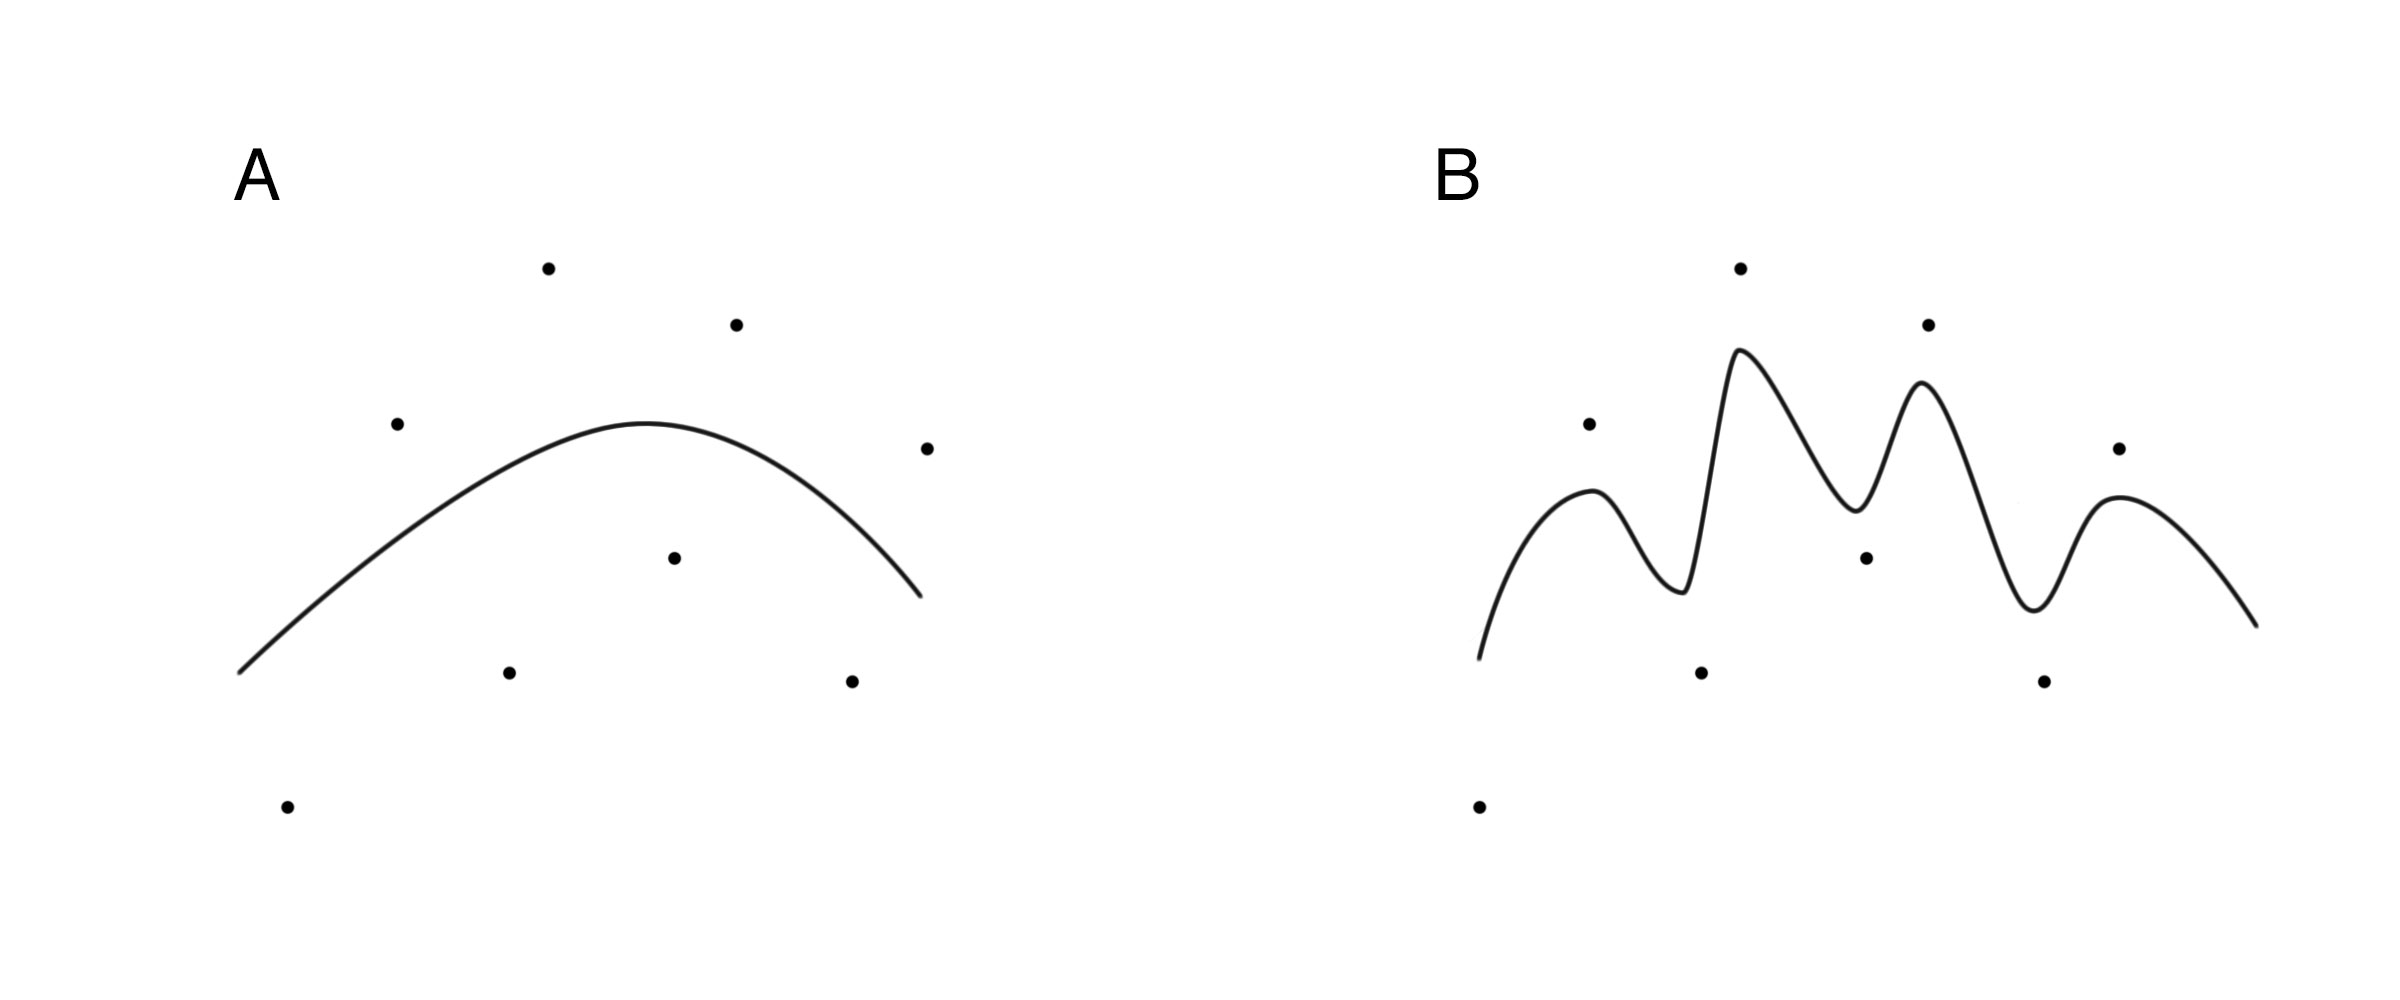
\includegraphics[width=0.99\linewidth,natwidth=898,natheight=587]{billeder/WP_000057.jpg}
\caption{A) Shows the generalized function. B) The approaching of output values}
\label{fig:WP}
\end{figure}
